\chapter{Simplicial Homology Global Optimisation}  \label{sec:shgo}
\section{Overview}
The SHGO method strongly relies on constructing a simplicial complex using the sampled points of an objective function $f$ as vertices. From this construction of the complex $\mathcal{H}$ we use the resulting directed subgraph which contains the set of all $1-$chains from the elements of $\mathcal{H}^1 \in \mathcal{H}$ to find minimiser pools using definitions similar to the methods demonstrated in the previous sections. This is accomplished by the application of Sperner's lemma \citep{Sperner1928} allowing us to approximate the domains of stationary points for any objective function in the feasible search space $\Omega$. 

It is proved that, if provided with an adequate sampling set, the construction of $\mathcal{H}$ will produce the same homology groups. This result is used to show that for the given sampling set of vertices $\mathcal{H}^0 \in \mathcal{H}$ we always extract the optimal minimiser pool similar to the one-dimensional case described in \Cref{sec:motivation}, but extended to higher dimensions. 

The algorithm itself consists of four steps which will be described in detail:
\begin{enumerate}
\item Uniform sampling point generation of N vertices in the search space within the bounded and constrained subspace of $\Omega$ from which the $0-$chains of $\mathcal{H}^0$ are constructed.
\item Construction of the directed simplicial complex $\mathcal{H}$ by triangulation of the vertices.
\item Construction of the minimiser pool $\mathcal{M} \subset \mathcal{H}^0$ by repeated application of Sperner's lemma.% and the Lefschetz Fixed Point Theorem.
\item Local minimisation using the starting points defined in $\mathcal{M}$.
\end{enumerate}

We will start by formally defining the construction of $\mathcal{H}$ from a given set of feasible sampling points $\mathcal{P}$ and proving its properties. %In this paper we will consider only a search space defined by a bounded hyperrectangle $\Omega \subseteq  [l, u]^n\subseteq\mathbb{R}^n$ with $\mathcal{P} \in \Omega$. It is easily extended to optimisation problems with simple linear constrains in $\mathbf{g}$ since the resulting space is compact and convex, however, care must taken if $\mathbf{g}$ contains non-trivial, non-linear constraints !!TODO: CITE NEW SECTION PROOF. In the practical implementation of the algorithm non-linear constraints can be defined, however, the properties defined here are not guaranteed.


\section{Directed simplicial complex approximation of the objective function}
Consider again the general objective function mapping in the continuous domain $f : \mathbb{R}^n \rightarrow \mathbb{R}$. The purpose of this section is to describe a discrete mapping $h: \mathcal{P}\rightarrow \mathcal{H}$ to provide a simplicial approximation for the surface of $f$. To guide the reader the methods will be demonstrated on the simple 2-dimensional optimisation problem defined in Example 4. The use of a 2-dimensional surface allows for a demonstration of the techniques while the abstractions defined are readily extended to higher dimensions. 

We start by formally defining the set of vertices from which $0$-chains of the simplicial complex are built and the of edges from which the $1$-chains of $\mathcal{H}$ are built.

\begin{definition} \label{def:h0}
Let  $\mathcal{X}$ be the set of sampling points generated by a sampling sequence in the bounded hyperrectangle $[\mathbf{l}, \mathbf{u}]^n$. The set $\mathcal{P} = \{\mathbf{x} \in \mathcal{X}~|~\mathbf{g}(\mathbf{x}) \geq 0 \}$ is a set of points within the feasible set $\Omega$ .
\end{definition}

\begin{definition} \label{def:h0.5}
For an objective function $f$, $\mathcal{F}$ is the set of scalar outputs mapped by the objective function $f:\mathcal{P} \rightarrow \mathcal{F}$ for a given sampling set $\mathcal{P} \subseteq \Omega \subseteq \mathbb{R}^n$.
\end{definition}

\begin{definition} \label{def:h1}
Let $\mathcal{H}$ be a directed simplicial complex. Then $\mathcal{H}^0 := \mathcal{P}$ is the set of all vertices of $\mathcal{H}$ .
\end{definition}

\begin{definition} \label{def:h2}
For a given set of vertices $\mathcal{H}^0$, the simplicial complex $\mathcal{H}$ is constructed by a triangulation connecting every vertex in $\mathcal{H}^0$. The triangulation supplies a set of undirected edges $E$.
\end{definition}

%\begin{definition} 
%For a given sampling set $\mathcal{P}$. The minimiser pool $\mathcal{M}$ is defined as 
%$\mathcal{M} = \{ \bold{p}^i~|~\forall j(f_j^{+i} > 0 	\land f_j^{-i} > 0), i = \{2, 3, \dots, N - 1\}\} \cup  \{ \bold{p}^i~|~\forall j(f_j^{-i} < 0), i = \{0\}\} \cup  \{ \bold{p}^i~|~\forall j(f_j^{+i} < 0), i = \{N\}\} $
%\end{definition}

\begin{definition} \label{def:h3}
The set $\mathcal{H}^1$ is constructed by directing every edge in $E$. A vertex $v_i \in \mathcal{H}^0$ is the connected to another vertex $v_j$ by an edge contained in $E$. The edge is directed as $\overline{v_i v_j}$ from $v_i$ to $v_j$ iff $f(v_i) < f(v_j)$ so that $\partial \left( \overline{v_i v_j} \right) = v_j - v_i$. Similarly an edge is directed as $\overline{v_j v_i}$ from $v_j$ to $v_i$ iff $f(v_i) > f(v_j)$ so that $\partial \left( \overline{v_j v_i} \right) = v_i - v_j$.
\end{definition}

For practical computational reasons we must also consider the case where $f(v_i) = f(v_j)$. If neither $v_i$ or $v_j$ is already a minimiser we will make use of rule that the incidence direction of the connecting edge is always directed towards the vertex that was generated earliest by the sampling point sequence. If $v_i$ is not connected to another vertex $v_k$ then we leave the notation $\overline{v_i v_k}$ undefined and let $\partial \left(\overline{v_i v_k}\right) = 0$. We let the higher dimensional simplices of $\mathcal{H}^k, k = 2, 3, \dots n + 1$ be directed in any arbitrary direction which completes the construction of the complex $h: \mathcal{P}\rightarrow \mathcal{H}$. We can now use $\mathcal{H}$ to find the minimiser pool for the local minimisation starting points used by the algorithm:

\begin{definition} \label{def:h4}
A vertex $v_i$ is a minimiser iff every edge connected to $v_i$ is directed away from $v_i$, that is $\partial \left( \overline{v_i v_j} \right) = (v_{j \neq i} - v_i) \lor 0~ \forall v_{j \neq i} \in \mathcal{H}^0$. The minimiser pool $\mathcal{M}$ is the set of all minimisers.
\end{definition}
%!!TODO: Be more explicit in defining $h$ precisely


We will also make extensive use of star notation \citep{Hatcher2011, Henle1979}:
\begin{definition} \label{def:h5}
The star of a vertex $v_i$, written $\textrm{st}\left( v_i \right)$, is the set of points $Q$ such that every simplex containing $Q$ contains $v_i$. \
\end{definition}
The $k-$chain $C(\mathcal{H}^k), k = n + 1$ of simplices in $\textrm{st}\left( v_i \right)$ forms a boundary cycle $\partial(C(\mathcal{H}^{n + 1}))$ with $\partial\left(\partial(C(\mathcal{H}^{n + 1}))\right) = \emptyset$. The faces of $\partial(\mathcal{H}^{n + 1})$ are the bounds of the domain defined by $\textrm{st}\left( v_i \right)$.

A visual demonstration of these constructions and notations is provided in the following numerical example:

\paragraph{Example 4} The Ursem01 function for two dimensions is defined as follows \citep{Gavana2016}
\begin{equation*}
\min f(\bold{x}) =  \displaystyle - \sin{\left(2 x_1  - 0.5 \pi \right) - 3 \cos{\left(x_2\right)}} - 0.5 x_1 , ~ x \in \Omega =  [0, 9] \times [-2.5, 2.5] 
\end{equation*}
\Cref{fig:ursem} provides a 3 dimensional plot of this function. The function has three local minima within the domain $\bold{x} \in [0, 9] \times [-2.5, 2.5]$.

\begin{figure} 
\centerline{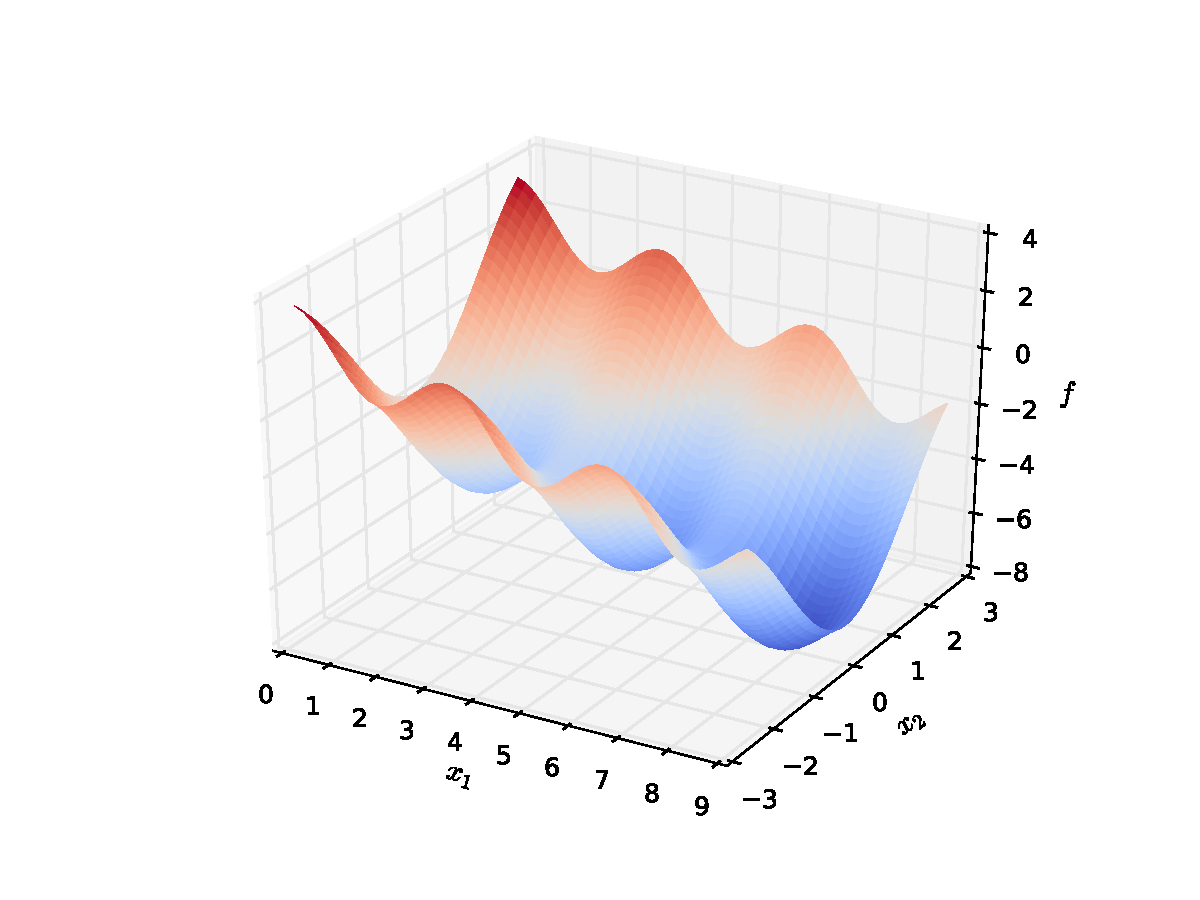
\includegraphics[scale=1.0]{./Fig6.pdf}}
{\caption{A 3-dimensional surface plot of the optimisation test function given in Example 4 $ f(\bold{x}) =  \displaystyle - \sin{\left(2 x_1  - 0.5 \pi \right) - 3 \cos{\left(x_2\right)}} - 0.5 x_1$ for the domain $\bold{x} \in \Omega = [0, 9] \times [-2.5, 2.5] $} \label{fig:ursem}}
\end{figure}

We use a set $\mathcal{P}$ of $N=15$ sampling points from the 2-dimensional Sobol sequence. First map out the objective function values:
\begin{equation} \label{eq:ursemmap}
f:
\begin{bmatrix} [l]
v_{0} = (0.0, -2.5) \\
v_{1} = (4.6, 0.0) \\
v_{2} = (6.9, -1.25) \\
v_{3} = (2.3, 1.25) \\
v_{4} = (3.45, -0.625) \\
v_{5} = (8.05, 1.875) \\
v_{6} = (5.75, -1.875) \\
v_{7} = (1.15, 0.625) \\
v_{8} = (1.725, -0.9375) \\
v_{9} = (6.325, 1.5625) \\
v_{10} = (8.625, -2.1875) \\
v_{11} = (4.025, 0.3125) \\
v_{12} = (2.875, -1.5625) \\
v_{13} = (7.475, 0.9375) \\
v_{14} = (5.175, -0.3125)  
\end{bmatrix}
\rightarrow
\begin{bmatrix} [l]
f_{0} = 3.403\\
f_{1} = -6.275\\
f_{2} = -4.0651\\
f_{3} = -2.208\\
f_{4} = -3.3429\\
f_{5} = -4.051\\
f_{6} = -1.493\\
f_{7} = -3.674\\
f_{8} = -3.591\\
f_{9} = -2.191\\
f_{10} = -2.606\\
f_{11} = -5.062\\
f_{12} = -0.601\\
f_{13} = -6.239\\
f_{14} = -6.044
\end{bmatrix}
\end{equation}

From \Cref{def:h1} we find $\mathcal{H}^0$ from $\mathcal{P}$. Next we use Delaunay triangulation to find a set of connected edges according to \Cref{def:h2}. Any triangulation scheme resulting in a simplicial complex can be used. Next the edges are directed from the calculated values of $\mathcal{F}$ using \Cref{def:h3}. Finally from \Cref{def:h4} we find the minimiser set $\mathcal{M} = \{v_{1}, v_{7}, v_{13}\}$. The resulting structure is shown in \Cref{fig:alp5}. Also shown in \Cref{fig:alp5} is the domain of $\textrm{st}\left( v_1 \right)$ for a visual description of \Cref{def:h5}. Next we increase the sampling size to $N = 150$ points and repeat the procedure. The resulting complex is shown in \Cref{fig:alp100}. Notice that while the minimiser vertices have changed (now closer to the true continuous local minima), the cardinality of the minimiser pool $|\mathcal{M}|$ remains unchanged. That is, given an adequate number sampling points $|\mathcal{M}|$ will cease to grow with increasing $N$, providing a heuristic for the number of sampling points needed to approximately map all minima of an objective function. This useful property of the SHGO algorithm is proven formally in \Cref{sec:invariance}. 

\begin{figure} 
\centerline{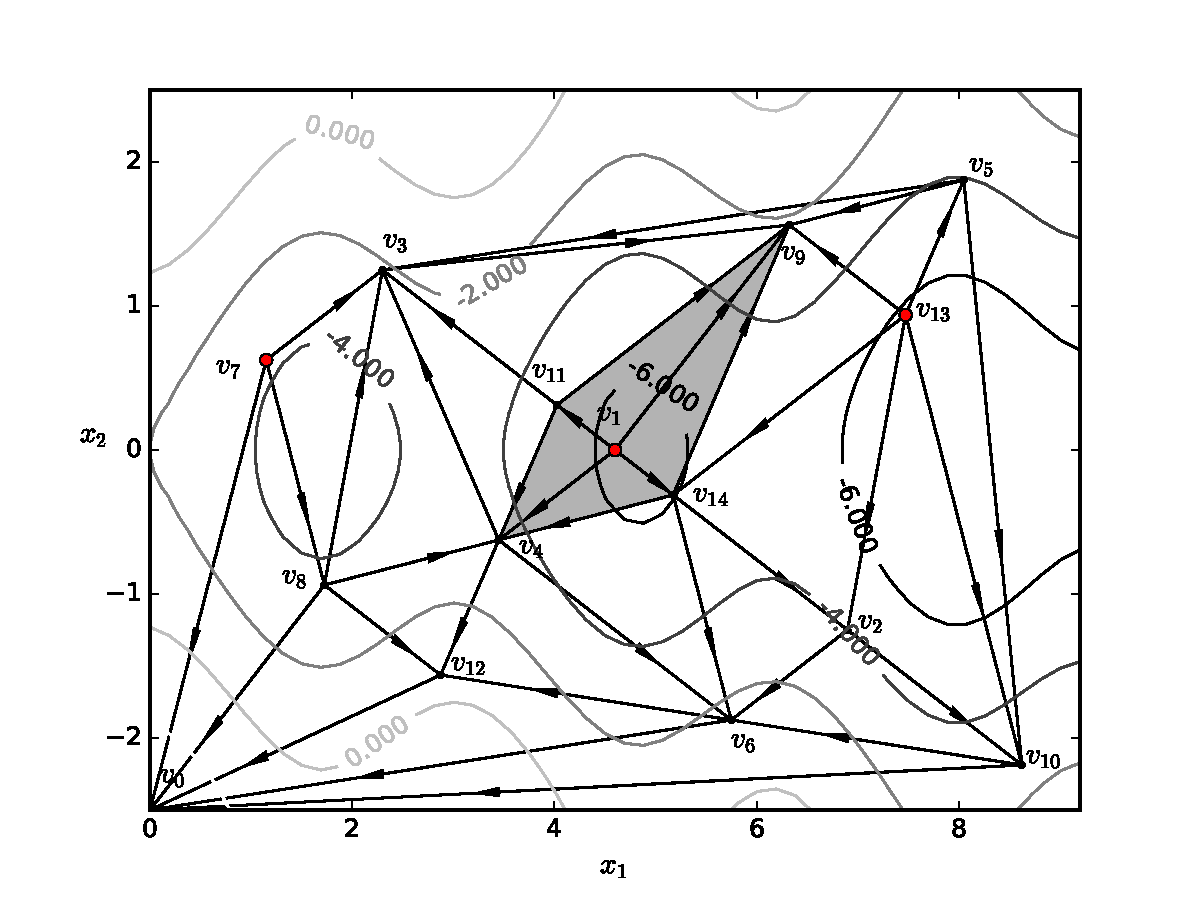
\includegraphics[scale=1.0]{./Fig7.pdf}}
{\caption{A directed complex $\mathcal{H}$ with $N=15$ forming a simplicial approximation for an objective function. There are three minimiser vertices $v_1$, $v_7$ and $v_{13}$ shown by the big red dots. The area shaded in grey represents the domain defined by $\textrm{st}\left( v_1 \right)$} \label{fig:alp5}}
\end{figure}

\begin{figure} 
\centerline{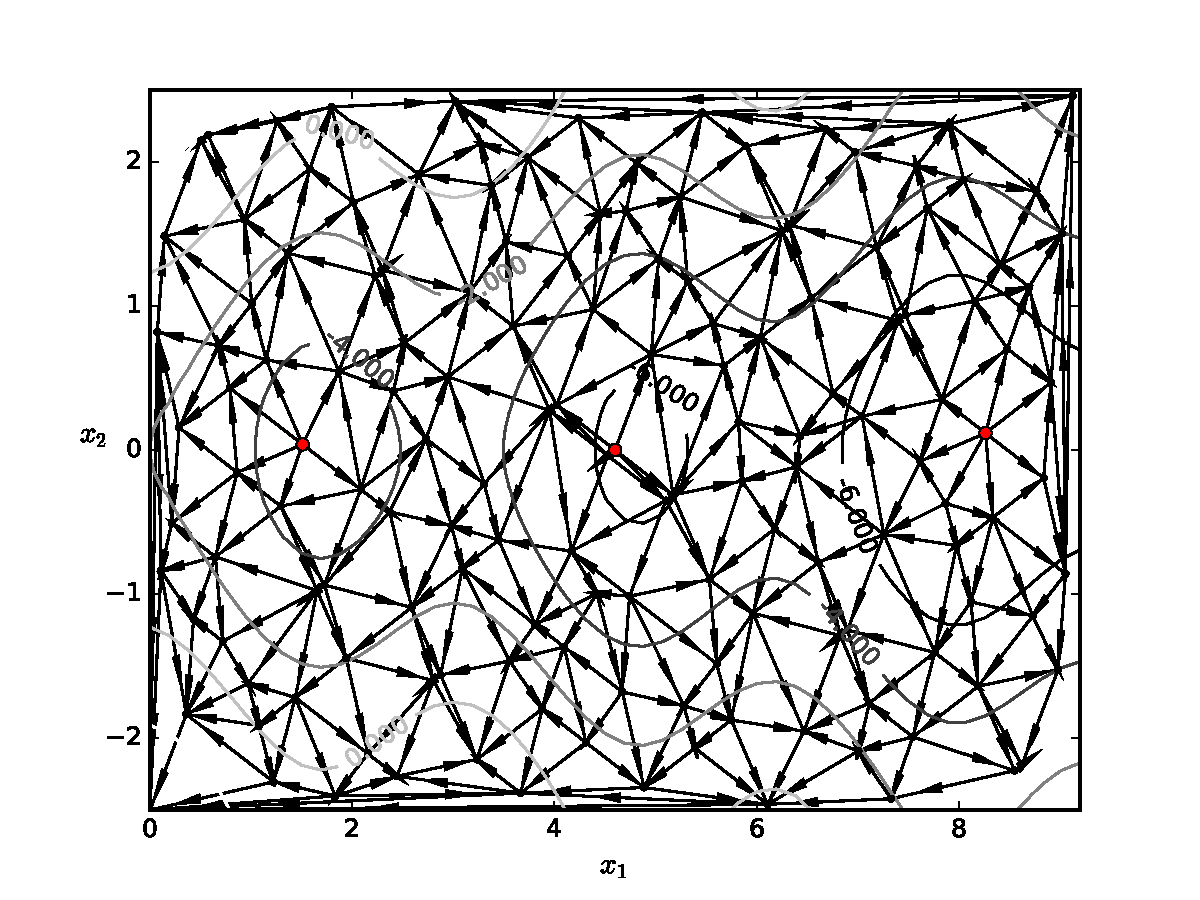
\includegraphics[scale=1.0]{./Fig8.pdf}}
{\caption{A directed complex $\mathcal{H}$ forming a simplicial approximation for an objective function with 150 vertices. There are three minimiser vertices given by the big red dots} \label{fig:alp100}}
\end{figure}

\section{Guarantee of stationary points in sub-domains near minimiser points}
This section is devoted to proving the following theorem:
\begin{theorem} \label{theor:stat}
%Given a minimiser $v_i \in \mathcal{M} \subseteq \mathcal{H}^0$ on the surface of a continuous, Lipschitz smooth objective function $f$ with a compact bounded domain in $\mathbb{R}^n$ and range $\mathbb{R}$. For any $n-$dimensional $k-$chain $C(\mathcal{H}^k), k = n + 1$ with subset of edges $E \subseteq \{C(\mathcal{H}^k), k = n + 1\}\subset \mathcal{H}^1$. If $v_i$ has incidence on a set of edges $E$, then the chain of simplices containing $E$ defines a $k-$chain $C(\mathcal{D}^k)$, $\mathcal{D}^k \subseteq \mathcal{H}^k$, $k=n+1$ near $v_i$ with every vertex in $C(\mathcal{D}^k)$ connected to $v_i$. There exists at least one stationary point of $f$ within the domain defined by the boundary cycle $\partial(\mathcal{D}^{n + 1})$.
Given a minimiser $v_i \in \mathcal{M} \subseteq \mathcal{H}^0$ on the surface of a continuous, Lipschitz smooth objective function $f$ with a compact bounded domain in $\mathbb{R}^n$ and range $\mathbb{R}$, there exists at least one stationary point of $f$ within the domain defined by $\textrm{st}\left( v_i \right)$.
\end{theorem}

\begin{proof}
Our strategy relies on finding a simplex with a Sperner labelling where each label represents a different $n + 1$ label in every vector direction of the gradient vector field $\nabla f$ of $f$ where of the $n + 1$ Cartesian directions we require only a vector pointing towards a section defined by $n + 1$ hyperplane cuts, the remainder of the proof then proceeds as usual for Brouwer's fixed point theorem \citep{Brouwer1911} found in for example \citet[p. 40]{Henle1979} utilising Sperner's lemma. Figure \ref{fig:spernerdemo} provides a visual example of a Sperner labelling of a 2-simplex for the reader's benefit. Figure \ref{fig:spernerfield} shows a geometrical example of how Brouwer applied this lemma on vector fields in his fixed point theorem.


\begin{figure} 
\centerline{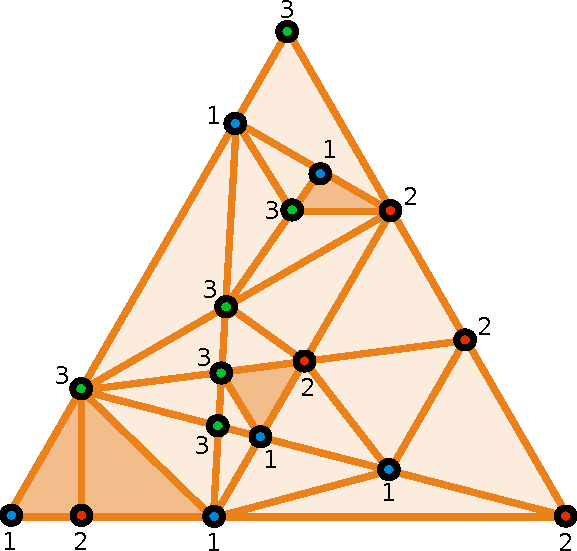
\includegraphics[scale=1.0]{./Sperner2d.pdf}}
{\caption{A Sperner labelling of a 2-simplex, every vertex of the n-simplex is labelled with a set of labels $1, 2, . . . , n + 1$. Any vertices on the boundary $(n-1)$-simplices of the n-simplex may only contain the labels of its boundary vertices  \label{fig:spernerdemo}}}
\end{figure}

\begin{figure} 
\centerline{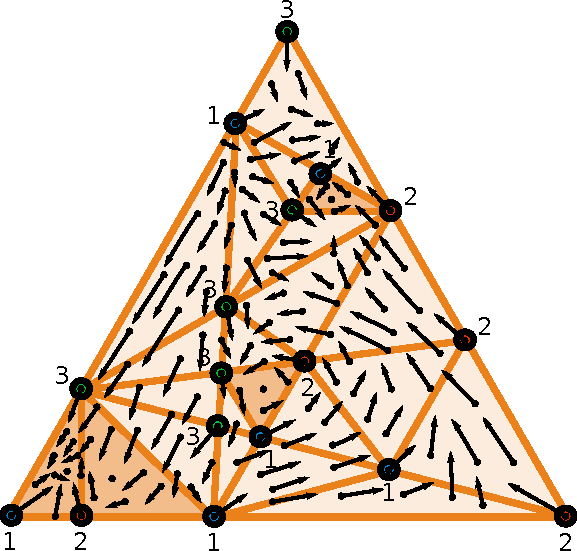
\includegraphics[scale=1.0]{./Sperner2d_vec.pdf}}
{\caption{A Sperner labelling applied by assigning directions in a vector field  \label{fig:spernerfield}}}
\end{figure}

\begin{theorem} (Sperner's lemma \citep{Sperner1928}) Every Sperner labelling of a triangulation of a n-dimensional simplex contains a cell labelled with a complete set of labels:  {1,2, \dots, n+1}.
\end{theorem}

Start with the observation that for any minimiser $v_i \in \mathcal{M} \subseteq \mathcal{H}^0$ we have by construction that for any vertex $v_j$ with incidence on a connecting edge $\overline{v_i v_j}$ that $f(v_i) < f(v_j)$, so by the MVT there is at least one point on $\overline{v_i v_j}$ where $\nabla f$ points towards a Cartesian direction in a section that can receive a unique Sperner label. If we have $n+1$ vertices with incidence on an edge $ \overline{v_i v_j}\subseteq \mathcal{H}^1$ in every required Cartesian direction then we have a simplex within $\textrm{st}\left( v_i \right)$ with a Sperner labelling. 

In the case where we do not have $n+1$ vertices in every required section then by construction there is no vertex between $v_i$ and the boundary of $f$ defined by $\Omega$ in the required section. In the case where the constraint is not active and there exists at least one point $v_k$ boundary where $\nabla f$ does not point towards the boundary and by the MVT $v_k$ can receive a unique Sperner label from which we can construct a simplex within $\textrm{st}\left( v_i \right)$ with Sperner labelling.

Following the combinatorial version of Brouwer's fixed point theorem \citep{Henle1979} since $\nabla f$ is continuous and the domain $\textrm{st}\left( v_i \right)$ is compact we can produce a sequence of complete triangulations with arbitrarily small size in which the size of the simplices decreases toward zero. This sequence produces a sequence of vertices with gradients $\nabla f(V)$ pointing in every $n+1$ direction. By continuity there is a vector $\nabla f (\mathbf{X})$ near the sequences, since the zero vector is the only vector pointing in all $n+1$ directions we have a point $\mathbf{X}$ bounded by the domain defined by $\textrm{st}\left( v_i \right)$ where $\nabla f (\mathbf{X}) = \bar{0}$.
In the case where the constraint is active a local minimum lies on the constraint which is in the domain defined $\textrm{st}\left( v_i \right)$. This concludes the proof.
% Start by approximating the gradient vector field of $f$ with the finite differences between the sampled set of vertices $\mathcal{H}_0$,% we denote the function $G(V)$ defined at every discrete vertex $v_i \subseteq \mathcal{H}_0$. The directed complex $\mathcal{H}$ provides a starting point described for Sperner labelling \citep{Musin2015} 
% remainder of proof proceeds as per \cite[p. 40]{Henle1979}
%TODO: Finish following Henle combinatorial proof for label $-->$ gradients $--> $ index theorem $--> $ stationary points.
\end{proof}

\Cref{fig:Sperner} provides a visual demonstration of the proof using the complex from Example 4. Here we have divided the plane so that the 3 required directions are $[0, \frac{\pi}{2})$, $[\frac{\pi}{2}, \pi)$ and $[\pi, 2 \pi)$. Note that this division is arbitrary and any $n + 1 = 3$ subdivisions can be chosen as long as all possible $n + 1 = 3$ directions can form a simplex in the space are covered. The three possible simplices are contained within the star domains of each minimiser $\textrm{st}\left(v_{1}\right)$, $\textrm{st}\left(v_{7}\right)$ and $\textrm{st}\left(v_{13}\right)$. 

First consider the minimiser $v_{13}$. There are three possible edges in $[\frac{\pi}{2}, \pi)$ on which a point exists that can be used as a vertex to receive a Sperner labelling for that direction namely $\overline{v_{13} v_{14}}$, $\overline{v_{13} v_{2}}$ and $\overline{v_{13}  v_{10}}$. The only possible edges in the $[0, \frac{\pi}{2})$, $[\frac{\pi}{2}, \pi)$ directions are $\overline{v_{13} v_{5}}$ and $\overline{v_{13} v_{9}}$ respectively. The simplex $\overline{v_{5} v_{9} v_{10}}$ drawn in \Cref{fig:Sperner} is not necessarily the simplex with a Sperner labelling. The three vertices of the Sperner simplex which are proven to exist through the MVT exists on each of the edges $\overline{v_{13} v_{14}}$, $\overline{v_{13} v_{2}}$ and $\overline{v_{13}  v_{10}}$ in a subdomain of this simplex $\overline{v_{5} v_{9} v_{10}}$. For example the simplex surrounding the minimiser $v_{1}$ is a possible Sperner simplex with vertices on the edges in every required direction.

\begin{figure}
\centerline{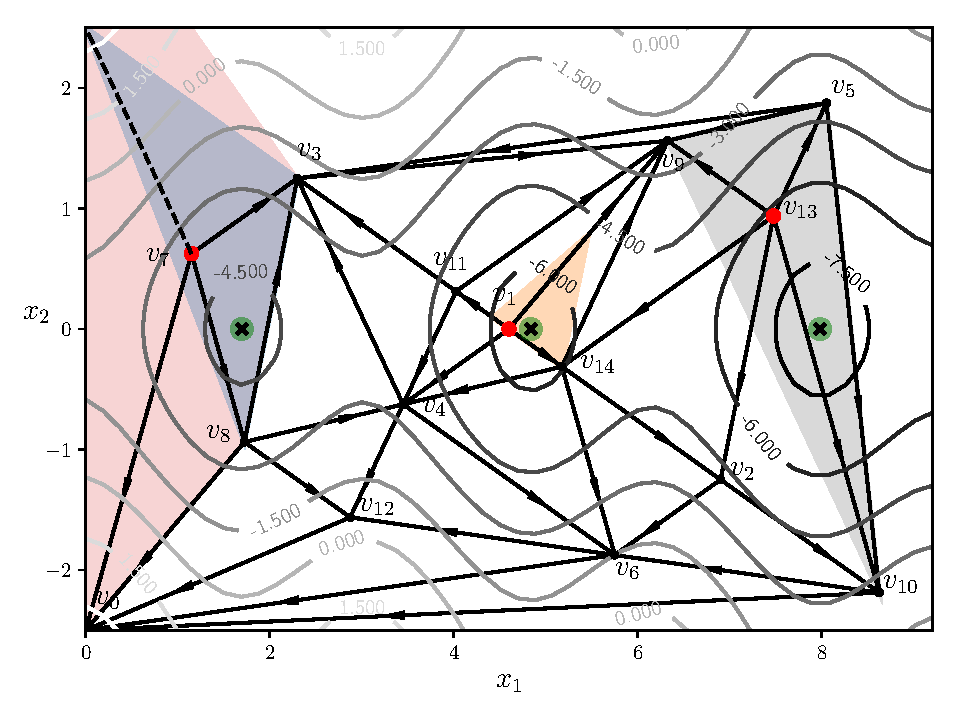
\includegraphics[scale=1.0]{./Fig9.pdf}}
{\caption{Visual demonstration of the proof by finding simplices with Sperner labellings. The three circled crosses are the (approximate) minimima of the objective function within the given bounds. The three possible Sperner simplices are contained within the star domains of each minimiser $\textrm{st}\left(v_{1}\right)$, $\textrm{st}\left(v_{7}\right)$ and $\textrm{st}\left(v_{13}\right)$. $v_{7}$ is an example of simplices without complete Sperner labelings, the red shaded area around $\overline{v_7}$ is the bounded domain wherein at least one local minimum exist
} \label{fig:Sperner}} 
\end{figure}

Note that if the edge $\overline{v_{13} v_{14}}$ was chosen instead of $\overline{v_{13}  v_{10}}$ then the local minimum of the function would be outside the domain of the simplex with the Sperner labelling. This is an important observation because it demonstrates that \Cref{theor:stat} cannot be used to further refine the location of the local minimum from the domain $\textrm{st}\left(v_{13}\right)$ using mechanisms of the proof, it only states that at least one local minimum exists within $\textrm{st}\left(v_{13}\right)$.

The boundaries of $\textrm{st}\left(v_{13}\right)$ can be found using the $3-$chain $C_{13}(\mathcal{H}^3)$ of simplices in $\textrm{st}\left( v_{13} \right)$, recall that the directions of simplices higher than dimension 2 are undefined and so the directions can be arbitrarily chosen $$C_{13}(\mathcal{H}^3) = \overline{v_{13} v_{10} v_{5}} + \overline{v_{13} v_{5} v_{9}} + \overline{v_{13} v_{9} v_{14}} + \overline{v_{13} v_{14} v_{2}} + \overline{v_{13} v_{2} v_{10}}$$

$C_{13}(\mathcal{H}^3)$ clearly forms a cycle, applying the boundary operator we find the faces defining the bounds of the domain of $\textrm{st}\left( v_i \right)$ which in this case is the chain of edges with defined direction  $$\partial(C_{13}(\mathcal{H}^{3})) = - \overline{ v_{10} v_{5}} + \overline{v_{5} v_{9}} - \overline{v_{9} v_{14}} + \overline{v_{14} v_{2}} + \overline{v_{2} v_{10}} $$ thus $\partial\left(\partial(C(\mathcal{H}^{3}))\right) = \emptyset$. 

$v_{7} = (1.15, 0.625)$ is an example of a minimiser that does not have all three required directions for a Sperner labelling, the light red shaded area represents the area wherein a local minimum can exist. For example on the lines $x_1 = 0$ for $x_2 \in [0.625, 2.5]$ or $x_2 = 2.5$ for $x_1 \in [0, 1.15]$ there will either exist a point $\bold{p}$ where the gradient $\nabla f (\bold{p})$ points in any direction pointing towards $[\frac{3}{2} \pi, 0)$ in which case and edge $\overline{v_{13} \bold{p}}$ exists that points in the $[\frac{\pi}{2}, \pi)$ direction and we have a simplex with a Sperner labelling. For example the dotted line on \Cref{fig:Sperner} with the Sperner simplex represented by blue shaded around $v_7$. If such a point does not exists then all points on those lines points in the $[0, \frac{3}{2} \pi)$ direction and so one or more local minimum lies somewhere on the boundary which is within the defined area.

%Note that while the extreme vertices where not sampled by the Sobol sequence (except for $v_0$), the bounds can be arbitrarily connected to the complex as was done with dotted edge connecting to $v_7$ to cover the entire search space.

It should be noted that in software implementations of shgo the boundaries of the star domain of a minimiser $\partial\left(\textrm{st}(v_1)\right)$ can be passed to any local optimisation routine that handles constraints constraints. Therefore, if the local minimisation routine is guaranteed to not produce an output outside the supplied bounds, then any iteration of shgo will not produce a solution outside the designated star domain for every minimiser.

There have been several developments in the extension of this lemma which could prove useful in applications extending the SHGO algorithm. One of the most interesting is by \citet{DeLoera2002} where they proved the Atanassov conjecture \citep{atanassov1996sperner} that for any polytope with $N$ vertices there are $N - n$ simplices that receive a complete set of Sperner labels. \citet{Meunier2006} further extended this theorem and more recently \citet{Musin2015} extended the theorems to a large class of manifolds with or without boundary. These theorems could prove useful for extending the algorithm to make use of this information. 
%More explicitly the Atanassov conjecture can be used to find how many stationary points exist in a domain larger than the simplices extracted from SHGO.
More explicitly, SHGO currently uses knowledge of the objective function evaluations, but only in a Boolean sense (in the form of directed edges). The theorems by Meunier and Musin allow us to extend Sperner's lemma to a simplicial complex built in a $(n+1)$-dimensional non-euclidean space. This would allow the application of ideas from discrete differential geometry. For example the Gauss-Bonnet theorem holds for discrete simplicial surfaces \citep{Crane2013DGP}. The Gauss-Bonnet theorem provides a relation between the total Gaussian curvature and the Euler characteristic of a surface. By simple summation of the angle defect around every vertex we can determine the Euler characteristic of a continuous surface. As will be demonstrated in Section 5.4 the simplicial complex used by SHGO is homeomorphic to complexes built on other topological hypersurfaces. Therefore when using explicit coordinates of the expected homomorphism the summation can be used to compare the error with the Euler characteristic which provides a metric for how accurately the objective function surface has been sampled. In global optimisation theory a simplicial complex built in this space can be used for approximating local and global Lipschitz constants for an objective function while still retaining the ability to detect locally convex sub-domains in the search space. %When the objective function is Lipschitz smooth ! discrete differential geometry \citep{Crane2013DGP}.





%%% Invariance
\section{Invariance of the directed complex within a bounded rectangle} \label{sec:invariance}

We now have a guarantee of finding stationary points in sub-domains near stationary points. However, we would also like to ensure that SHGO does not generate more than one minimiser starting point per convex sub-domain. This can only be guaranteed when an objective function surface is "adequately sampled". For black box functions there is no way to know if the number and distribution of sampling points is adequate without more information (for example if the number of local minima are known in the problem). However, it is an important property of the algorithm that $|\mathcal{M}|$ will stop increasing with higher sampling after this point. First we define an adequately sampled surface.

\begin{definition}
Consider a simplicial complex $\mathcal{H}$ built on an objective function $f$ with a compact feasible set $\Omega$ using Definitions \ref{def:h1} through \ref{def:h4}. The surface is said to be \bf{adequately sampled} \normalfont if there is one and only one true stationary point within every domain defined by \Cref{theor:stat}.
\end{definition}

The remainder of this section is devoted to proving the following theorem which holds in the case where $\Omega = [\mathbf{l}, \mathbf{u}]^n$.

\begin{theorem} \label{theorem:invariance_M} (Invariance of an adequately sampled simplicial complex $\mathcal{H}$) For a given continuous objective function $f$ that is adequately sampled by a sampling set of size $N$. If the cardinality of the minimiser pool extracted from the directed simplex $\mathcal{H}$ is $|\mathcal{M}|$. Then any further increase of the sampling set $N$ will not increase $|\mathcal{M}|$.
\end{theorem}

\begin{proof}
The proof relies on a homomorphism between the simplicial complex $\mathcal{H}$ constructed in the bounded hyperrectangle $\Omega$ and the homology (mod 2) groups of a constructed surface $\mathcal{S}$ on which we can invoke the invariance theorem.

Define the $n$-torus $\mathcal{S}_0$ from the compact, bounded hyperrectangle $\Omega$ by identification of the opposite faces and all extreme vertices. Now for every strict local minimum point $\bold{p} \in \Omega$ puncture a hypersphere and after appropriate identification the resulting $n$-dimensional manifold $\mathcal{S}_g$ is a connected g sum of g tori $S := S_0\,\#\,S_1\,\#\,\cdots\,\#\,S_{g - 1} \qquad  (g\text{ times})$.

For the reader's benefit Figures \ref{fig:stori} and \ref{fig:stori_sum} demonstrates the process geometrically. Figure \ref{fig:stori} shows how to puncture a hypersphere and make the usual identifications in a 2-dimensional problem.  Figure \ref{fig:stori_sum} demonstrates the construction of $\mathcal{S}_g$.


\begin{figure} 
\centerline{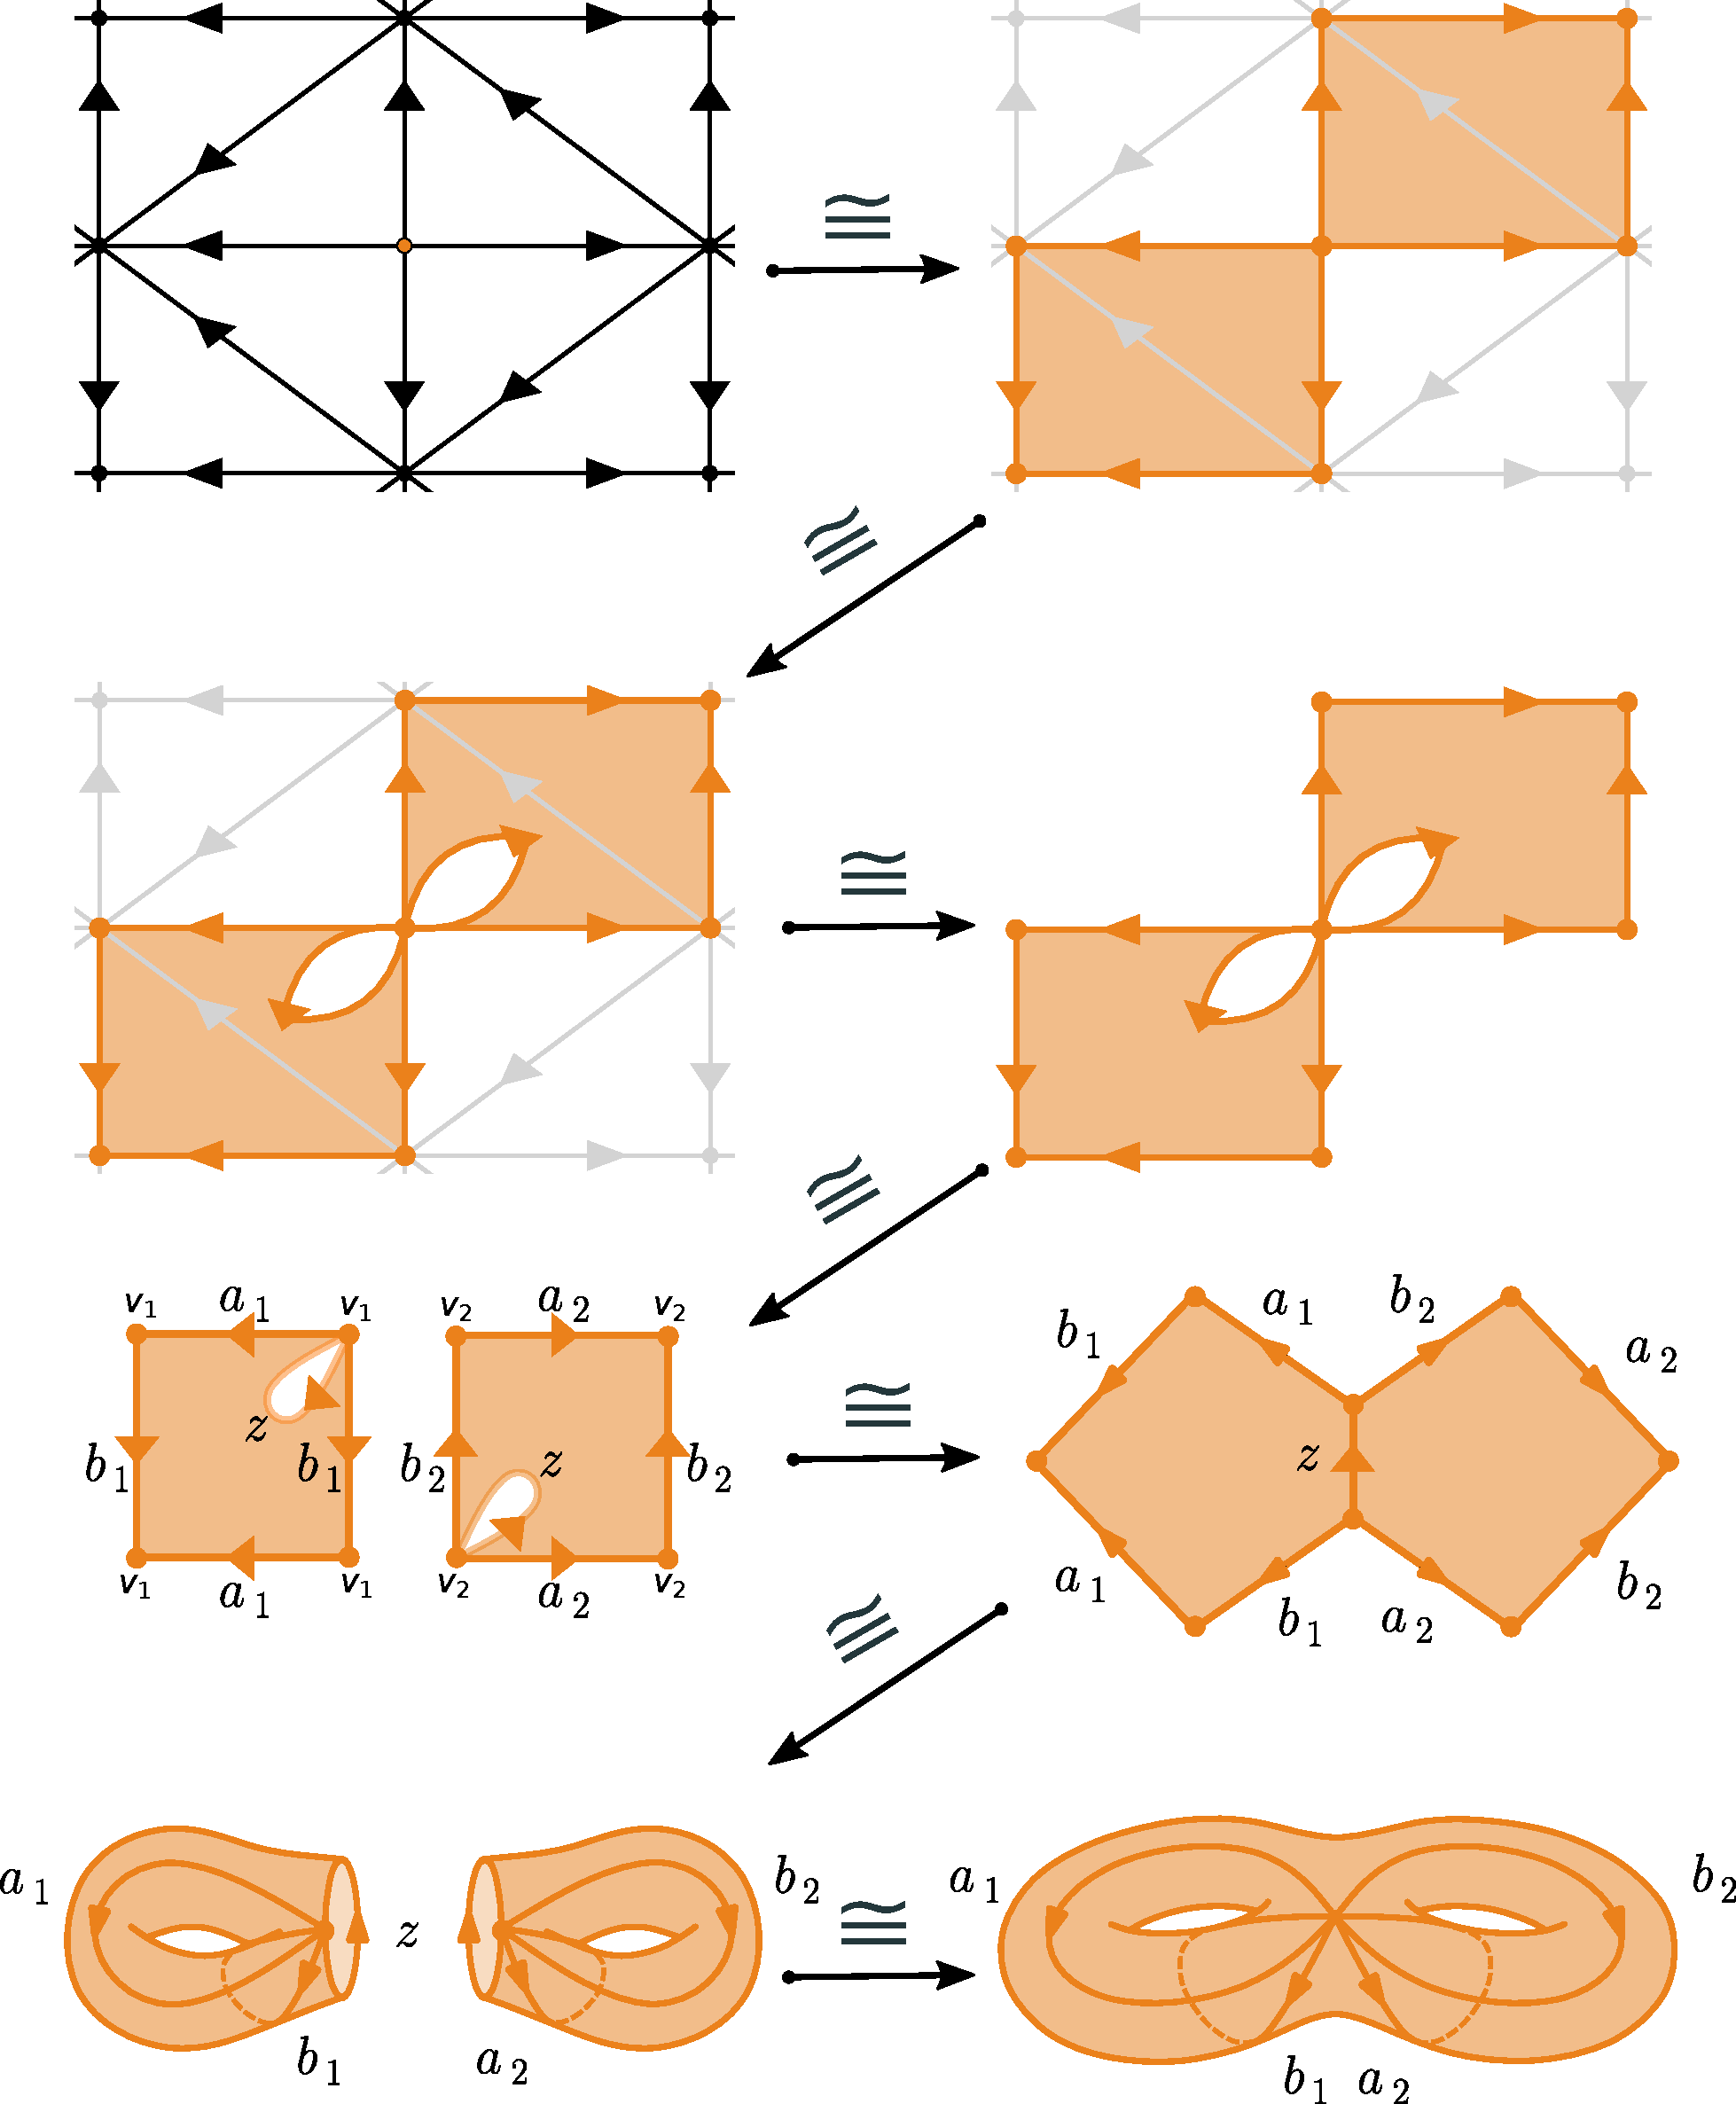
\includegraphics[scale=0.5]{./stori_complete.pdf}}
{\caption{The process of puncturing a hypersphere at a minimiser point in a compact search space. Start by identifying a minimiser point in the $\mathcal{H}^1$~($\cong~\mathcal{K}^1$) graph. By construction, our initial complex exists on the (hyper-)surface of an $n$-dimensional torus $\mathcal{S}_0$ such that the rest of $\mathcal{K}^1$ is connected and compact. We puncture a hypersphere at the minimiser point and identify the resulting edges (or ($n-1$)-simplices in higher dimensional problems). Next we shrink (\it a topoligical (ie continuous) transformation\normalfont) the remainder of the simplicial complex to the faces and vertices of our (hyper-)plane model. Make the appropriate identifications for $\mathcal{S}_0$ and glue the identified and connected face $z$ (a ($n-1$)-simplex) that resulted from the hypersphere puncture. The other faces (ie ($n-1$)-simplices) are connected in the usual way for tori constructions)\label{fig:stori}}}
\end{figure}

\begin{figure} 
\centerline{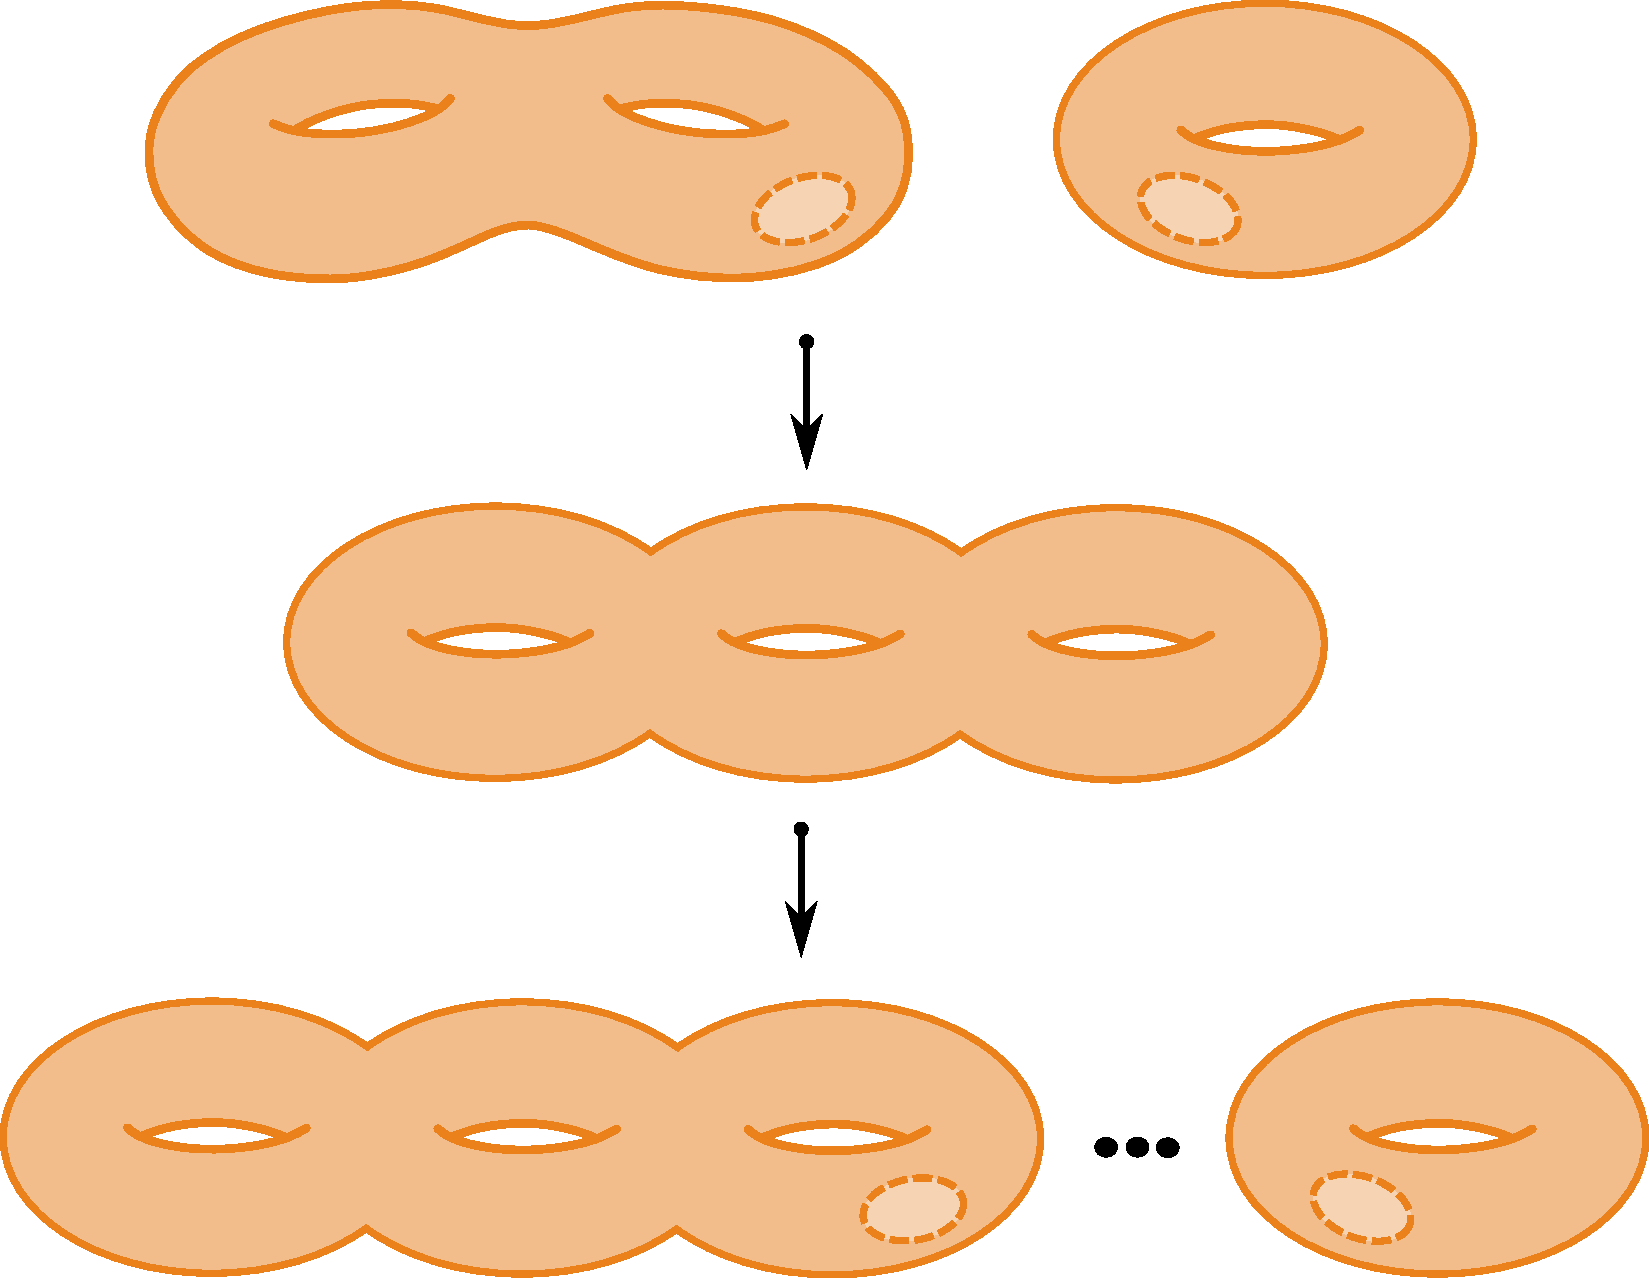
\includegraphics[scale=0.4]{./stori_sum.pdf}}
{\caption{The process of puncturing a new hypersphere on $\mathcal{S}_0\,\#\,\mathcal{S}_1$ can be repeated for any new minimiser point without loss of generality producing $S := S_0\,\#\,S_1\,\#\,\cdots\,\#\,S_{g - 1} \qquad  (g\text{ times})$ \label{fig:stori_sum}}}
\end{figure}


Any triangulation $\mathcal{K}$ of the topological space $\mathcal{S}$ is homeomorphic to $\mathcal{S}$, $\bold{H}_k(\mathcal{K}) \cong \bold{H}_k(\mathcal{S}) ~\forall k \subset \mathbb{Z}$. Note that this homomorphism is for a mod 2 homology between a triangulation $\mathcal{K}$ and the surface $\mathcal{S}$ and is thus undirected. A triangulation corresponding to all vertices and faces of $\mathcal{K}$ can be directed according to \Cref{def:h1}, \Cref{def:h2} and \Cref{def:h3} providing the directed simplicial complex $\mathcal{H}$. By construction we have, for an adequately sampled simplicial complex $\mathcal{H}$, an equality which exists between the cardinality of $\mathcal{M}$ and the Betti numbers of $\mathcal{S}$ as $|\mathcal{M}| = h_1 = \text{rank} (\bold{H}_1(\mathcal{S})) = \text{rank} (\bold{H}_1(\mathcal{K}))$. Here we invoke the invariance theorem

\begin{theorem} (Invariance theorem\citep{Henle1979}) %(Henle p. 154) 
The homology groups associated with a triangulation $\mathcal{K}$ of the a compact, connected surface $\mathcal{S}$ are independent of $\mathcal{K}$. In other words, the groups $\bold{H}_0 (\mathcal{K})$, $\bold{H}_1 (\mathcal{K})$ and $\bold{H}_2 (\mathcal{K})$ do not depend on the simplices, incidence coefficients, or anything else arising from the choice of the particular triangulation $\mathcal{K}$; they depend only on the surface $\mathcal{S}$ itself.
\end{theorem}
The invariance theorem can be extended to higher dimensional triangulable spaces using singular homology through the Eilenberg-Steenrod Axioms \citep{eilenberg47foundations, Henle1979}. As a direct consequence any triangulation of $\mathcal{S}$ will produce the same homology groups for $\mathcal{K}$.

Adding any new sampling point within the corresponding subdomains of $\textrm{st}\left( v_i \right)$ $ \forall i (v_i \in \mathcal{M} \subseteq \mathcal{H}^0 ) $ as defined in \Cref{theor:stat} will by Definitions \ref{def:h1} through \ref{def:h4} need to be connected directly to $v_i$ by a new edge or the triangulation is no longer a simplicial complex and thus not increase $|\mathcal{M}|$ since only one vertex will be the new minimiser.

After adding any sampling point outside a domain $\textrm{st}\left( v_i \right)$ then, through the established homomorphism, any construction of $\mathcal{H}$ will produce the same homology groups since $\text{rank}(\bold{H}_1(\mathcal{K}))$ remains unchanged and it is thus not possible for a new vertex to be wrongly identified as a minimiser in the triangulation $\mathcal{H}$.

This concludes the proof that any increase in $N$ will not further increase $|\mathcal{M}|$.
\end{proof}

It is important to note that \Cref{theorem:invariance_M} is only applicable to complexes with adequate sampling as defined, that is to say it is entirely possible that, in complexes with less that adequate sampling, two starting minimiser elements of $\mathcal{M}$ will converge to the same local minimum. This flaw is inherent in the fact that there is insufficient information to completely identify the minima of a surface (and could be overcome if some extra information about $f$ is known).

%The set of sampling vertices $\mathcal{H}_0$ is directly related to the complex $\mathcal{F}$ by the boundary operator in the obvious way $\Omega \overset{\partial}{\leftarrow } \mathcal{F}_1 \overset{\partial}{\leftarrow } \mathcal{F}_2 \dots \overset{\partial}{\leftarrow } \mathcal{F}_n$. By puncturing the minimisers (formally defined as the toroidal points of the directed graph $\mathcal{F}_1$) in $\mathcal{F}$ a homomorphism to the homology (mod 2) groups $\mathcal{F}_k \cong\mathcal{H}_k ~\forall k \subseteq \mathbb{Z}$ can be formed which can be used as an approximate characterisation of the objective function $f$. An iterative procedure is used to apprimate the characterisation to a preset tolerance.

\Cref{theor:stat} and \Cref{theorem:invariance_M} also lead to the following corollary about an optimisation problem:

\begin{corollary} \label{corollary:smooth}
Consider any objective function $f : \Omega \subseteq \mathbb{R}^n \rightarrow \mathbb{R}$. Consider also a local minimisation routine that is guaranteed to converge to a local minimum in the same locally convex domain as the starting point inputted to the algorithm. Alternatively the local minimisation routine is guaranteed to converge to a point within a set of bounds (provided by the boundary of the $k$-chain around $\textrm{st}\left( v_i \right)$,  $\partial \left( C(\mathcal{H}^k) \right), ~k = n + 1$). If such a local minimisation routine  uses an element $v_i \in \mathcal{M}$ as a starting point and the routine leads to a minimum outside or on $\textrm{st}\left(v_{i}\right)$ and in addition the minimum is not contained in the set $\mathcal{H}^0$. Then it can be concluded that either search space is not adequately sampled or $f$ is not a Lipschitz smooth function.
\end{corollary}
Therefore according to \Cref{corollary:smooth} if the number of local minima are known, as in for example phase equilibria problems, then we can extract valuable information about the objective function. In particular it can be determined whether or not the objective function is Lipschitz smooth. Alternatively if the function is known to be Lipschitz smooth then \Cref{corollary:smooth} can be used to prove the sampling is insufficient when the condition is not met. When this happens it is also now known that there are more local minima to be found, one or more of which might possibly be the global minimum. \Cref{corollary:smooth} does not, however, provide any guarantee that the sampling is sufficient when the conditions are met.
